% !TEX root = /Users/kquine/Dropbox/Research/Papers/2015/CPS-SMT-RTSS/cps-rtss.tex

\section{Preliminaries on PALS}
\label{sec:pals}

PALS transforms 
 a \emph{synchronous design} $\mathit{SD}$ with  period $T$
into a %\emph{correct-by-construction} 
distributed real-time system $\mathcal{MA}(\mathit{SD}, T, \Gamma)$
that satisfies the same temporal logic ($CTL^*$) formulas,
provided that the underlying 
infrastructure guarantees bounds %$\Gamma$ on network delays, execution times,  and clock skews, 
$\Gamma = (\epsilon, \alpha_{\min}, \alpha_{\max}, \mu_{\min}, \mu_{\max})$
with
%
\begin{inparaenum}[(i)]
	\item $\epsilon$ a maximal clock skew  with respect to the global clock,
	\item $[\alpha_{\min},\alpha_{\max}]$  bounds for processing
          I/O and 
	executing a transition,   %%%  , and real-time scheduling
	and
	\item $[\mu_{\min}, \mu_{\max}]$ bounds  for the network transmission delay.
	%between any two nodes. % in the network.
\end{inparaenum}
This section overviews the synchronous models, % $\mathit{SD}$,
the distributed  models, % $\mathcal{MA}(\mathit{SD}, T,\Gamma)$,
 and their relationship %between $\mathit{SD}$ and $\mathcal{MA}(\mathit{SD}, T,\Gamma)$
(we refer to~\cite{mr-pals-journal,pals-tcs} for details).


\subsection{Discrete Synchronous Models}

The synchronous model $\mathit{SD}$ is specified  as 
an \emph{ensemble}
$\mathcal{E}$  of %(nondeterministic)
state machines with input and output ports.
In  each iteration, a machine performs a transition
based on its current state and its inputs, %or its environment)
 proceeds to the next state, and generates new outputs for the next iteration.


\begin{definition}
A  \emph{typed machine}  $M = (D_i,S,D_o,\delta_M)$
is composed of:
%
\begin{inparaenum}[(i)]
	\item $D_i = D_{i_1} \times \cdots \times D_{i_n}$ an input set 
	(a value to the $k$-th \emph{input port}  is an element of  $D_{i_k}$), 
	% for $1 \leq k \leq n$, 
	\item $S$ a set of states, 
	\item $D_o =D_{o_1} \times \cdots \times D_{o_m}$ an output set,
	% (a value from the $j$-th \emph{output port} is an element of  $D_{o_j}$)
        and 
	% for $1 \leq j \leq m$
	\item $\delta_M \subseteq (D_i \times S) \times (S \times D_o)$ a total
	transition relation.
\end{inparaenum}  
\end{definition}




As illustrated in Fig.~\ref{fig:ensemble},
a collection $\{M_j\}_{j\in J_S\cup J_F}$ of  state machines with different periods 
can be composed into a 
\emph{multirate ensemble} $\mathcal{E}$.
The period of a slow machine $s \in J_S$ (with $\mathit{rate}(s) = 1$) is 
a multiple of the period of a fast machine $f \in J_F$ (with $\mathit{rate}(f) > 1$). 
A \emph{wiring diagram}, which has no connections between two fast
machines,  connects the  input ports and output ports of the machines.

\begin{figure}
\centering
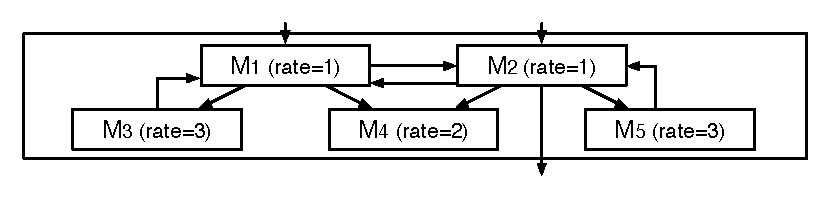
\includegraphics[clip=true,trim=0.3cm 0.4cm 0.3cm 0.4cm,width=\columnwidth]{ensemble.pdf}    
\caption{A multirate ensemble $\mathcal{E}$,
with $M_1$ and $M_2$ slow machines.
%and $M_3$, $M_4$, and $M_5$ are fast machines.
}  \label{fig:ensemble}
\end{figure}

In each iteration, all components in $\mathcal{E}$ perform a
transition each \emph{in lockstep}.
A fast machine $f$ is \emph{slowed down} 
and performs $k = \mathit{rate}(f)$ \emph{internal} transitions  in one global synchronous step.
Since 
a fast machine produces $k$-tuples of outputs in one step, 
%but a slow machine only needs  a single input value.
%Therefore,
\emph{input adapters} are used 
to generate single values (e.g., the last value, or 
the average of the $k$ values) for a slow machine. 
Likewise, a single output  from a slow machine is adapted to a $k$-tuple of inputs 
for a fast machine.




The \emph{synchronous composition}  of a multirate ensemble $\mathcal{E}$
is equivalent to a single machine $M_\mathcal{E}$.
If a machine in $\mathcal{E}$ has a feedback wire connected to itself or to another component, then the output becomes an input of the destination component in the next iteration.
That is,  $M_\mathcal{E}$'s states %$S^{\mathcal{E}} = (\Pi_{j\in J} S_j) \times (\Pi_{j\in J}  D_\mathit{OF}^j)$,
consist of the states %$S_j$ 
of its subcomponents %$M_j$ 
and
the   ``feedback'' outputs. %$D_\mathit{OF}^j$ for $j \in J_S \cup J_F$
%(i.e., the outputs from  $M_j$   to some machine in $\mathcal{E}$). 
For example, 
%the synchronous composition 
$M_\mathcal{E}$ of 
%the ensemble 
$\mathcal{E}$ in Fig.~\ref{fig:ensemble} 
is the machine given by the outer box. 
%Notice that $M_\mathcal{E}$ can appear as a component 
%in another multirate ensemble, resulting in hierarchical multirate systems.

%\textbf{(Peter) I have to add some discussion about the environments  and their timelessness ...}

The global \emph{environment} can be modeled as another typed
machine, and \emph{local} environments are assumed to be composed with their
controllers into a single typed machine. 
This model is an untimed model (apart from the period $T$): 
the result of applying a (controller or environment) transition is 
independent of \emph{when}  the transition is applied in a round. 

\subsection{PALS Distributed  Real-Time Models}
\label{pals-dist}

Each component in the  distributed model $\mathcal{MA}(\mathcal{E}, T, \Gamma)$
is composed of a machine in $\mathcal{E}$ and \emph{wrappers} around it, as illustrated in Fig.~\ref{fig:wrappers}.
%The outermost wrapper  is  the PALS wrapper, which encloses an input adaptor wrapper, 
%which  encloses either a (slow) machine or a $k$-machine wrapper, 
%which encloses a  (fast) machine. 
In $\mathcal{MA}(\mathcal{E}, T, \Gamma)$,
each machine performs at its own rate according to its local clock.
%that deviates by less than $\epsilon$ from the global  clock.
At the beginning of its periods, it reads its input from the layer above, 
performs a transition, and then generates the outputs.
%when the execution of the transition is finished.

\begin{figure}
\centering
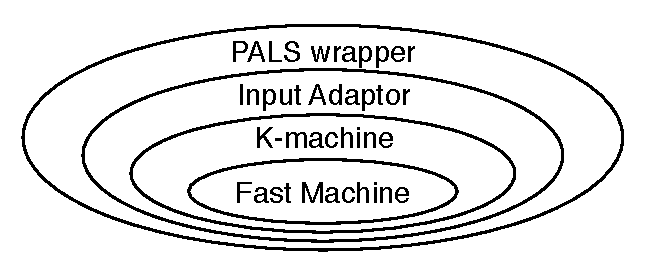
\includegraphics[width=0.49\columnwidth,clip=true,trim=0.3cm 0.3cm 0.3cm 0.3cm]{Onion-f.pdf}
\hfill
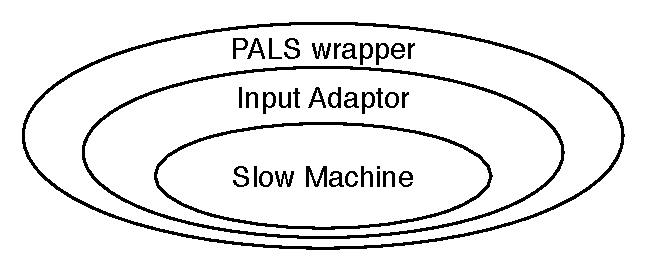
\includegraphics[width=0.49\columnwidth,clip=true,trim=0.3cm 0.3cm 0.3cm 0.3cm]{Onion-s.pdf}
\caption{The wrapper hierarchies %for fast machines (left) and slow machines (right) 
in PALS distributed real-time  models.}
\label{fig:wrappers}
\end{figure}


%
A wrapper has I/O buffers,  timers, and access to the machine's  local clock.
Each PALS wrapper %communicates with the other components, and 
has the same \emph{global period $T$} and stores 
received inputs  in its input buffer.
When the $i$-th round begins %according to its local clock 
(at time $u_0 \in (iT-\epsilon, iT+\epsilon)$),
it delivers the contents of its input buffer to the inner input adaptor wrapper,
and sets its \emph{backoff timer} to $2\epsilon -\mu_{min}$.
%to prevent that outputs are sent out too early.
When the execution of the inner components is finished \emph{and}
the backoff timer expires, % (before $u_0 + \max(2\epsilon -\mu_{min}, \alpha_{max})$),
the contents of the output buffer are sent out.% into the network, and
\footnote{The outputs are sent out before $u_0 + \max(2\epsilon -\mu_{min}, \alpha_{max})$,
and delivered to the destination before $u = \mu_{max} + u_0 +  \max(2\epsilon -\mu_{min}, \alpha_{max})$.
Therefore, if $T\geq 2\epsilon + \mu_{max} + \max(2\epsilon -\mu_{min}, \alpha_{max})$,
then all inputs are read in a round-consistent way since $u < (i+1)T - \epsilon$ \cite{pals-tcs}.}
%%% Kyungmin: my understanding is that we give a brief overview of
%%% Multirate PALS here; we do not try to _justify_ its correctness
%%% here.
%%% That has been done elsewhere.  Therefore, I suggest 
%%% that we skip the details about why it works, especially
%%% since many of the details do not seem to be used much later in the
%%% paper. 



An input adaptor wrapper reads the inputs from the PALS wrapper
and applies input adaptors %function
%to get either a single value from a $k$-tuple input  for slow machines, or
%a $k$-tuple of values from a single input for fast machines.
for each global period $T$. % according to its local clock.
A  $k$-machine wrapper
\begin{inparaenum}[(i)]
	\item extracts each value from the $k$-tuple input and delivers it to the enclosed fast machine
at each fast period $T/ k$, and
	\item delivers the $k$-\emph{tuples} from the outputs of the fast machine to its outer layer
	at each global period $T$.
\end{inparaenum}



A fast machine $M_f$ %in $\mathcal{MA}(\mathcal{E}, T, \Gamma)$ 
may \emph{not} be able to finish 
all of its $k$ internal transitions in a global  round
 \emph{before} the outputs must be sent to arrive before %the beginning of 
the next round.
The number of transitions that $M_f$ can perform before the deadline is 
 $k'= 1+\lfloor \max(T - (2\epsilon + \mu_{max} + \alpha_{max_f}), 0)\cdot (k / T)\rfloor$,
 where  $\alpha_{{\max}_f}$ is the maximal execution time for $M_f$.
If $k' < k$,
then $M_f$'s $k$-machine wrapper only sends the first $k'$ values
(followed by $k - k'$ ``don't care'' values $\bot$).
The input adaptor of each %slow machine's 
input port whose source is $M_f$
must %be \emph{$(k'+1)$-oblivious}, i.e., it 
ignore the last $k - k'$ values
$v_{k'+1}, \ldots, v_k$ in a $k$-tuple $(v_1, \ldots,  v_k)$.
%


\begin{figure}
\begin{center}
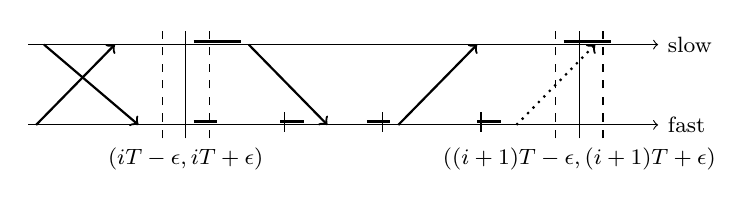
\begin{tikzpicture}[yscale=0.85,font=\footnotesize]
\draw [->] (0,0) -- (8,0) node  [right] {fast};
\draw [->] (0,1.2) -- (8,1.2) node [right] {slow};

\draw (2, -0.2) node [below] {$(i  T - \epsilon, i T + \epsilon)$} -- (2, 1.4);
\draw[dashed] (1.7, -0.2) -- (1.7, 1.4)  ;
\draw[dashed] (2.3, -0.2)  -- (2.3, 1.4);

\draw (7, -0.2) node [below] {$((i+1)  T - \epsilon, (i+1) T + \epsilon)$} -- (7, 1.4);
\draw[dashed] (6.7, -0.2)  -- (6.7, 1.4);
\draw[dashed] (7.3, -0.2)  -- (7.3, 1.4);

\draw [->,thick] (0.1, 0) -- (1.1, 1.2);
\draw [->,thick] (0.2, 1.2) -- (1.4, 0);

\draw [->,thick] (2.8, 1.2) -- (3.8, 0);
\draw [->,thick] (4.7, 0) -- (5.7, 1.2);
\draw [->,thick,dotted] (6.2, 0) -- (7.2, 1.2);

\draw [very thick] (2.1, 1.25) -- (2.7, 1.25);
\draw [very thick] (6.8, 1.25) -- (7.4, 1.25);

\draw [very thick] (2.1, 0.05) -- (2.4, 0.05); 
\draw [very thick] (3.2, 0.05) -- (3.5, 0.05); \draw (3.25, -0.1) -- (3.25, 0.2);
\draw [very thick] (4.3, 0.05) -- (4.6, 0.05); \draw (4.5, -0.1) -- (4.5, 0.2);
\draw [very thick] (5.7, 0.05) -- (6.0, 0.05); \draw (5.75, -0.1) --(5.75, 0.2);

\end{tikzpicture}
\caption{Timeline for $\mathcal{MA}(\mathcal{E}, T, \Gamma)$ ($k=4$ and $k' = 3$).
Diagonal arrows denote network transmission and short horizontal lines denote the execution.
The dotted arrow illustrates that the outputs can arrive after the beginning of the next round 
%for the slow component 
if the fast machine waits until all its transitions are finished.
\label{fig:mr-timeline}}
\end{center}
\end{figure} 



\subsection{Relating the Synchronous and Distributed Models}

In  $\mathcal{MA}(\mathcal{E}, T, \Gamma)$,
network transmission can happen only in the time interval  $(iT+\epsilon, (i+1)T-\epsilon)$
for each $i$-th period, as depicted in Fig.~\ref{fig:mr-timeline}.
Therefore, at each time $iT - \epsilon$, all the input buffers of the PALS wrappers are full, 
and all the other input and output buffers are empty.
A \emph{stable state} of the distributed model $\mathcal{MA}(\mathcal{E}, T, \Gamma)$
is a snapshot of the system at each time $iT - \epsilon$,
just before the components in $\mathcal{MA}(\mathcal{E}, T, \Gamma)$ 
start performing local machine transitions \cite{pals-tcs}.



\emph{Big-step} transitions are defined between two stable states of $\mathcal{MA}(\mathcal{E}, T, \Gamma)$,
and they are related to single steps of the synchronous composition
$M_{\mathcal{E}}$ through the 
%
  function $\mathit{sync}$ 
associating to each stable state  the corresponding state in  $M_{\mathcal{E}}$.
%
Two stable states are related by $s_1 \sim_\mathit{obi} s_2$ iff 
their  machine states are identical
and 
their corresponding input buffer contents \emph{cannot} be
distinguished by input adaptors.  

\begin{theorem}\label{thm:mr-pals}   \cite{mr-pals-journal}
The relation $(\sim_\mathit{obi} \,;\, \mathit{sync})$ 
is a bisimulation between 
the transition system induced by $M_{\mathcal{E}}$
and the big-step stable transition system induced by $\mathcal{MA}(\mathcal{E}, T, \Gamma)$.
\end{theorem}










